\section{Versuchsdurchführung}
\subsection{Versuchsaufbau}
Die verwendete Versuchsapparatur besteht aus einer Kupfer-Röntgenröhre, einem LiF-Kristall mit verstellbarem Kristallwinkel und einem darum drehbar gelagerten Geiger-Müller-Zählrohr. Für die Messung von Absorptionsspektren kann ein Absorber des zu messenden Materials vor dem Zählrohr platziert werden. Die Messelektronik ist im Gerät integriert, sodass die Messparameter wie Kristallwinkel, Drehmodus und Integrationszeit der Messung auf einem Computer festgelegt werden können.
\subsection{Überprüfung der Bragg-Bedingung}
Zur Überprüfung der Bragg-Bedingung wurde bei einem fest eingestellten Kristallwinkel von $\theta=14°$ der Winkel des Zählrohres in $0,1°$-Schritten variirt. Dies wurde im Intervall von $26°$ bis $30°$ unter einer Integrationszeit von $t=5s$ durchgeführt.
\subsection{Emissionsspektrum}
Das Emissionspektrum der Kupfer-Röntgenröhre wurde mit einer Integrationszeit von $t=10s$ unter Variation des Kristallwinkels von $\Delta \Theta=0,1°$ gemessen.
\subsection{Absorptionsspektren}
Für die Absorptionsmessung wurden die entsprechenden Absorber vor dem Zählrohr platziert und anschließend unter  
\begin{figure}
    \centering
    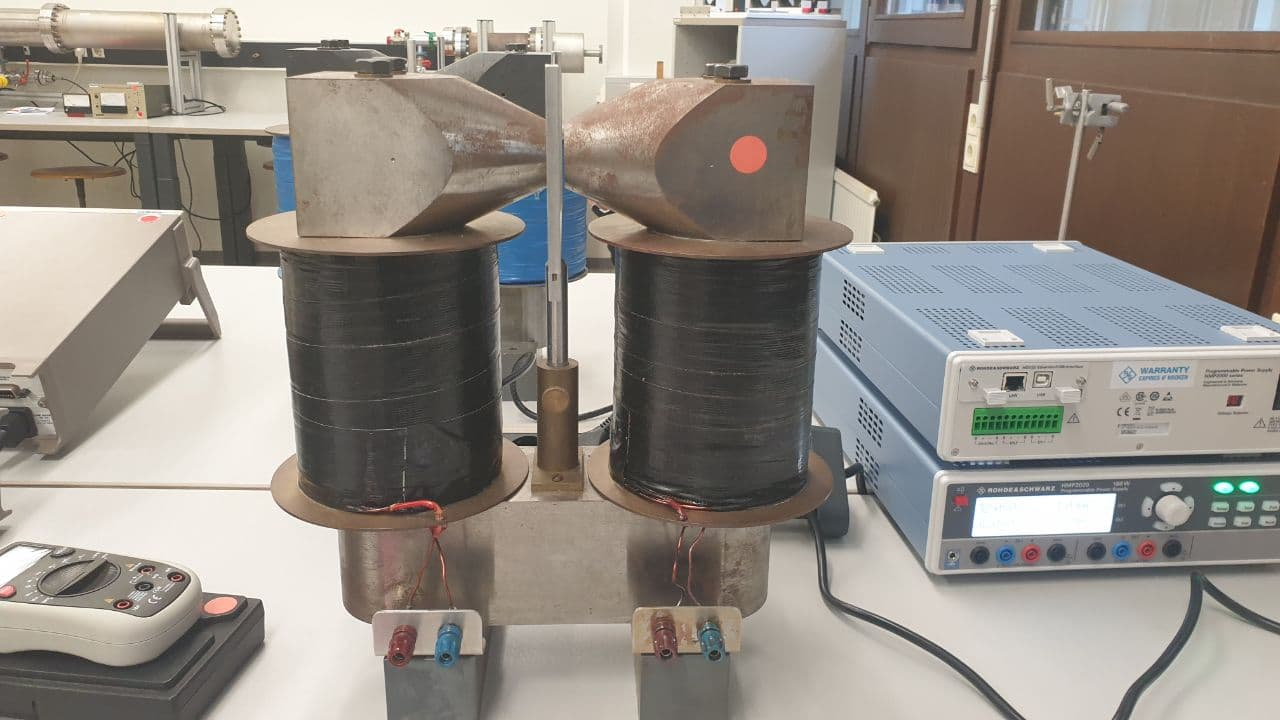
\includegraphics[width=10cm]{magnet.png}
    \caption{Elektromagnet}
    \label{fig:emagnet}
  \end{figure}

  
